%% -*- coding: utf-8-unix -*-

% \begin{lstlisting}[caption=,label=lst:]
% \end{lstlisting}

\chapter{テストシナリオ実装}
\label{chap:poc-scenario-dev}

PoCで実施したテストシナリオの実装、実際にテスト自動化をおこなってわかっ
たことや注意事項などについて解説する。

 \section{テストシナリオの概要}

  \subsection{ネットワークテストの方針}

\ref{chap:poc-target-design}章で設定したとおり、\yo ネットワークのテスト
を考える。そのためのテストシナリオとして「静的なふるまいのテスト」「動的
なふるまいのテスト」の2種類を実装する。テストシナリオ実装・テスト実行を
通して、物理ネットワークのテスト自動実行のポイント検討や問題点の抽出、従
来の人手によるテスト作業との比較をおこなう。

  \subsection{BDDテストシナリオの基礎}
  % - TDD/BDDとBDDツールとしてのCucumber
  % - Narrative
  % - ネットワークテストを書く上での検討点、今回のプロジェクトでの方針・決めごと
  %   - なぜそうきめたのか?

      \paragraph{テストツール}
NetTesterはテスト用ノードの生成・テスト対象ネットワークへの配置(パッチ接
続)をおこなうためのAPIを提供する。提供されるAPIを使用して \yo ネットワー
クのテストを実装する。\footnote{実際に作成した自動テストのためのコードは
NetTester Examples~\cite{nettester-ex}として公開している。}

テストシナリオの記述については、アプリケーションのテストでつかわれる既存
のツールと連携することを想定している。本PoCでは、「BDDによるネットワーク
のテスト」を考えていること(\ref{sec:behavior-test}節)、広く使われている
ツールであること、RubyベースでNetTesterとの親和性が高いことをもとに、BDD
ツールであるCucumber\cite{cucumber}を採用した。

    \paragraph{Narrative}
    % Cucumber の .feature の書き方 – NetTester
    %   https://3.basecamp.com/3088280/buckets/867009/messages/155991347
    % クライアントの要望にこたえるWebサービス開発 ~「らせん型ワークフロー」のススメ~
    %  http://www.slideshare.net/mayuco/css-nite-in-sapporo-vol5-14085124
BDDでは、テストのストーリー(フィーチャ)を以下のような構造で記述する
\cite{rspec-book,spiral-workflow}。
\begin{description}
 \item[タイトル] どのストーリーについて説明するのかを示す。タイトルは一
            般に、ユーザがシステムに要求するかもしれないアクティビティを
            短い言葉で表したものになる。
 \item[ナラティブ] ストーリーの内容について説明をする。一般的には
            Connextraフォーマットと呼ばれる形式の短い文章で記述される。
            このテンプレートは、誰がシステムを使っていて、そのユーザは何
            をしていて、なぜそのことに関心があるのか、を明確にする。
            \begin{itemize}
             \item ``As a (role)'': [誰のために(role)]として
             \item ``I want (feature)'': [何を(feature)]したい
             \item ``So that (bussiness value)'': なぜなら[なぜ
                   (bussiness value)]のためだ
            \end{itemize}
 \item[受け入れ基準] ストーリーの完了・完成を定義する受け入れ基準、シナ
            リオの定義。
\end{description}

Cucumberにおけるフィーチャとは、システムを利用するユーザーまたは別のコン
ピュータの視点に立っておおまかに表現された要件のことを指す。Cucumberの
フィーチャはタイトルと簡単なナラティブ、受け入れ基準としての役割をはたす
自動化されたシナリオによって構成される。
\begin{itemize}
 \item フィーチャはタイトルとナラティブで構成され複数のシナリオを含む。
       (本プロジェクトでは\verb|features/*.feature|ファイル)
       \begin{itemize}
        \item シナリオはそれぞれ、シナリオ内でおこることを任意のステップ
              で記述する。
       \end{itemize}
 \item 個々のステップ定義は開発で使っているシステムの言語で記述される。
       (本プロジェクトではRuby: \verb|features/step_definitions/*.rb|ファ
       イル)
\end{itemize}

% Narrative を Pull Requst する – NetTester
%   https://3.basecamp.com/3088280/buckets/867009/todos/159223633
% NetTester機能拡張(NW機器間接続)方針・やりたいこと – NetTester
%   https://3.basecamp.com/3088280/buckets/867009/todos/182746431
% Firewall の cucumber シナリオ – NetTester
%   https://3.basecamp.com/3088280/buckets/867009/todos/158299550

 \section{静的なふるまいのテスト}
% テストシナリオ策定の考えかた…そもそもなにをするテストなのか。どのような
% 検討を経てテストシナリオをきめたのか。narrativeの定義のプロセスとか。
% TODO: OOD資料にかいたようなテストコード解説のはなしをこちらにも含めるか?
% - 実装
%   - Step2テスト業務で気づいたことをまとめる – NetTester
%     \url{https://3.basecamp.com/3088280/buckets/867009/todos/260220903}

  \subsection{テストとして実現したいこと}
ネットワークに対して最低限要求されることは、ネットワークを介して必要な通
信が実現できることである。ネットワークの目的は、大きく言えばコミュニケー
ションを実現することである。あるノードが、他のノードと、必要な手段(アプ
リケーション)で通信できるかどうか、という点がまず初めにネットワークに求
められる機能要求となる。

「ネットワークの静的なふるまい」(\ref{sec:behavior-to-test}節)では、ネッ
トワークが定常状態にある(一定の状態にあって状態変化しない)ときに、ネット
ワーク利用者が実現したいend-to-endの通信がすべて実現可能かどうかをテスト
する。

  \subsection{テスターに求められる機能}

テストで確認したいend-to-endの通信、すなわち、実現したい通信要求は、通信
をおこなうノード(エンドポイント)の論理的・物理的な配置の組合せに応じて異
なる。また、通信をおこなうアプリケーションによっても別途制御がおこなわれ
る。例えば、DPIをおこなうFWやLBなどがネットワーク内にある場合は、単純な
宛先(ヘッダ)情報だけではなく、やりとりされるアプリケーションレベルの情報
によって通信の可否などが変化する。

したがって、単純なend-to-endの通信試験だとしても、配置やアプリケーション
の組合せによって大量のテストケースが発生してしまう、テストのためのリソー
ス確保などが充分にできない、などの課題があった
(\ref{sec:discuss-network-test}節)。

そこで、テスター(NetTester)では以下の機能が要求される。
\begin{itemize}
 \item テスト用ノードの生成
 \item テスト用ノードの配置
 \item テスト用ノード上でのタスク実行
 \item 複数のテスト用ノード操作/集中管理
\end{itemize}
NetTesterはこうしたノードの生成・配置・集中制御の機能(API)を提供している。
テストシナリオ(Cucumber)ではBDDの考えかたに基づいて、ノード間でどういっ
た通信を実現する必要があるかを個別の通信要件
(\ref{sec:network-requirements}節)ごとに定義する。

  \subsection{静的なふるまいのテストで実際に発見できた問題点}
  \label{sec:statictest-founded-issues}

静的なふるまいのテストでは、\yo ネットワーク通信要件
(\ref{sec:network-requirements}節)それぞれについてテストシナリオを実装し、
個々の要件に対してend-to-endの通信試験が自動化できることを実証した。テス
トの実行によって実際に発見できた物理ネットワークの問題点について解説する。

   \subsubsection{テスト対象ネットワークの設定不備の発見}
 % DNSのテスト作る – NetTester
 % https://3.basecamp.com/3088280/buckets/867009/todos/301325453
 % 通信要件\#29 B社PC→DMZ内のVPNサーバの疎通確認(SSLVPN) – NetTester
 % https://3.basecamp.com/3088280/buckets/867009/todos/233178490

 % 通信要件\#10 A社内PC→インターネットの疎通確認(ICMP) – NetTester
 % https://3.basecamp.com/3088280/buckets/867009/todos/233175867
 % 通信要件#27インターネット→ファイアウォールの疎通確認(ICMP) – NetTester
 % https://3.basecamp.com/3088280/buckets/867009/todos/233178319

一般的な(人手による)疎通試験と同様に、pingやその他のアプリケーションによ
る通信確認によって、テスト対象ネットワーク上の不備(要求される仕様と異な
る)点あるいはそれにつながる事象を発見できた。

    \paragraph{テスト対象ネットワークの設定ミス}
テスト対象ネットワークを構築した際の設定ミスによる問題を発見した。主要な
ものはFWのパケットフィルタルールの設定不備、NAT(NAPT)の設定ミスによるも
のである。これらは「できなければいけないこと」ができていない(テストが失
敗する)ことによって発見されたものである。以下に例を示す。
\begin{itemize}
 \item インターネットからNAT(VIP)を経由してDMZへアクセスする通信失敗(パ
       ケットフィルタルールの設定漏れ)
 \item \yo 内部ゾーンから外部ゾーン(internet)への通信失敗(NAPT設定ミス)
 \item FWが持つIPに対するping失敗(FWデフォルトのping応答ポリシ設定漏れ)
\end{itemize}

    \paragraph{テスト作業者側(構築・運用側)の通信仕様の認識違い}
登場人物(\ref{sec:poc-casting}節)に示したように、テストシナリオの実装や
実行をおこなった担当者は必ずしもネットワークやネットワーク機器のスペシャ
リストではない。そのため、FWのゾーン間通信についてのFWのポリシの認識不足
\footnote{ゾーン間通信のデフォルトポリシについて、当該機器を使用したこと
があるネットワークエンジニアとしては自明だったために明確に伝達がおこなわ
れていなかった。}から、\yo 外部ゾーン(インターネット)から内部ゾーンへの
ping通信が可能と判断してテストシナリオを実装してしまったケースがあった。
実際には要件どおり設定されたFWによってこのテストが失敗し、認識違いがあっ
たことが判明した。

   \subsubsection{ネットワーク機器の動作不具合}
   \label{sec:find-nw-device-bug}
 % 原因切り分けメモ (muraki) – NetTester
 % https://3.basecamp.com/3088280/buckets/867009/documents/217782147
 % 調査: テスト環境でシナリオ実行すると2回目以降でコケる – NetTester
 % https://3.basecamp.com/3088280/buckets/867009/todos/218486066

当初、静的なふるまいのテストのテストシナリオを実装し、動作させたときに、
同一のテストシナリオが実行されるたびに成功・失敗をくりかえすという事象が
あった。調査したところ、FWのARP処理の挙動について以下のような動作をして
いることがわかった。
\begin{itemize}
 \item NetTesterが生成するテスト用ノードでは、IPアドレスは一定だが、MAC
       アドレスはテストシナリオ実行ごとにランダムに変更する。
 \item FWにARP前のシナリオで実行したテスト用ノードのMACエントリが残って
       いると、次のシナリオで実行した(IPは同一だがMACアドレスが異なる)ARPに
       対して応答しない。(ARPエントリのクリアをおこなっても応答しない。)
 \item FWのARPエントリをクリアして、クライアントからTCP通信をおこなって
       もFW(Gateway)からサーバ側へのARPが確認できず、MACアドレスを学習し
       ていないにもかかわらず TCP SYN が送信されることがある。
\end{itemize}

これらの事象および当初使用していたFWのOSバージョンが古かったことから、
FW(OS)の不具合と判断し、FWのOSを更新する
\footnote{\tabref{tbl:device-list}参照。FWは更新版6.3.0r22.0(2016/4月リ
リース)に対して当初は6.3.0r5.0(2010/9月リリース)を使用していた
\cite{screenos-releases}。}ことで解決した。

   \subsubsection{L7レベルのFW挙動変化}
今回のテストシナリオ実装では、当初L4レベルの通信確認から実装し、可能なも
のについては実際のサーバ/クライアントを使用したL7レベルでの実装をおこなっ
ている。L4レベルの通信確認としては、netcat を使った任意の TCP/UDP port
listenとクライアントからの接続(tcpセッション確立/単純なサーバからの応答
確認)を使用している。L7レベルのend-to-endテスト実装としては以下のシナリ
オがある。
\begin{itemize}
 \item インターネットへのSSLアクセス(openssl, curlを使用したテストシナリ
       オ実装
       \footnote{\url{https://github.com/net-tester/examples/blob/feature/ood_demo/features/step_definitions/google_steps.rb}})
 \item SSHサーバヘのアクセス(opensshを使用したテストシナリオ実装
       \footnote{\url{https://github.com/net-tester/examples/blob/feature/ood_demo/features/step_definitions/ssh_steps.rb}})
 \item DNSサーバへのアクセス(dnsmasqを使用したテストシナリオ実装
       \footnote{\url{https://github.com/net-tester/examples/blob/feature/ood_demo/features/step_definitions/dns_steps.rb}})
\end{itemize}

特に、DNSのテストについては、当初 netcat によるL4レベル確認として実装し
たが、テストが成功しなかった(FWを経由して通信ができなかった)。今回使用し
たFW(SSG)の詳細なフィルタ仕様については調査していないが、このとき
\code{dig}コマンド等による実際の名前解決はできていたことから、テストシナ
リオとしてもdnsmasqによるL7レベルでのトラフィック生成シナリオを実装して
いる。

 \section{動的なふるまいのテスト}
% 障害試験シナリオを書く – NetTester
% \url{https://3.basecamp.com/3088280/buckets/867009/todos/238169066}
% Step2to3タスク検討
% https://drive.google.com/open?id=0B2eRR_JxYJA5M1RGdEZaOFkxTFk

  \subsection{テストとして実現したいこと}
  \label{sec:dynamic-test-target}
% NetTester機能拡張検討
% https://drive.google.com/file/d/0B2eRR_JxYJA5TmhaeWItNF93Um8/view
ネットワークは状況に応じて状態を変化させる。変化のトリガとして、例えば障
害発生による冗長経路への切替、メンテナンスのための一部のデバイスの停止や
切り離し・そのための通信経路迂回、ネットワーク機器の追加(拡張)や削除(縮
小)などがある。こうしたイベントに対して、ネットワーク(全体)は、ネットワー
クの状態と発生したイベントに応じて自らの情報(状態)を自律的に更新し、トラ
フィックの経路を変更するなどの制御をおこなう。

「ネットワークの動的なふるまい」(\ref{sec:behavior-to-test}節)では、ネッ
トワークが状態変化するときに、ネットワーク利用者へ与える影響が許容範囲内
かどうかをテストする。ネットワーク利用者への影響とは、ネットワーク状態遷
移中に発生するトラフィックの継続可否、影響度・影響範囲(場所的な範囲や時
間)である。例を以下にあげる。
\begin{itemize}
 \item トラフィックの継続可否
       \begin{itemize}
        \item ロードバランサなどL7の情報にしたがってトラフィックを操作す
              るような機器では、冗長系切替のときに、セッション情報などを
              引きついでアプリケーション通信を維持することが求められる。
              同様にNATなどの変換テーブルに基づいてトラフィックを操作す
              る機器でも冗長系機器間で状態の同期が必要になる。
        \item 系切替には隣接する機器も関連する。例えば、対象とする冗長系
              のL1/L2の切替に Gratuitous ARP を使用する機器で、隣接する
              L2スイッチのバグによって Gratuitous ARP 処理が正しくおこな
              われず、全体としてトラフィックの継続に失敗した事例などがあ
              る。
       \end{itemize}
 \item 影響度・影響範囲
       \begin{itemize}
        \item 状態変化によって予期しない現象が予期しない範囲でおこること
              がある。範囲としては、物理的な場所(特定のスイッチの配下な
              ど)・論理的な場所(特定のL2セグメントなど)複数の要素が考え
              られる。
        \item 仮想化によって物理構成と論理構成は分離されることが一般的で
              ある。この際、物理構成操作のオペミスや論理構成操作ミス(記
              述ミスや勘違い)の見落としがセグメント全体をまきこむL2ルー
              プを引き起すことがある。
        \item 機器のバグや設定ミス、そのほかの機能との併用による機器CPU
              専有状況の発生などがあると、こうした系切替によるトラフィッ
              クの維持・継続ができなかったり、想定した時間内に完了できな
              いことがある。例として、多数のVLANを収容していたL3スイッチ
              で、系切替の際のSTPトポロジ再計算処理によるCPU専有が発生し、
              スイッチ配下のセグメント全域で広範囲にわたって切替時間の遅
              延・それにともなうトラフィックの維持失敗(タイムアウト発生)
              がおこってしまった事例などがある。
       \end{itemize}
\end{itemize}

いくつか事例を挙げたが、これらの問題はネットワーク全体(系全体)の相互作用
に影響される。ネットワークの場合はベンダや機器ごとに独自のOSやアーキテク
チャを持つものが多く、特定機能や製品を組み合わせたときの相性問題やキャパ
シティ問題、特定ハードウェアやソフトウェア(バージョン)のトラブルといった
情報を共有することは難しい。また、複数の冗長化機能(複数の機器にまたがる
ものも含む)の連動する際、状態遷移のタイミングなどで機能単体では問題なく
動作する機能が複合した結果、問題が発生することもある\footnote{例として:
OSPF/BGP収束時間差によるブラックホールやループの発生
\cite{j3g14-packet-forwarding}など。}。こうした理由により、ネットワーク
の操作・状態変化において、すべての影響を予想するのは非常に困難である。

動的なふるまいのテストでは、上に挙げた「トラフィックの継続可否」「影響度・
影響範囲」のテストを自動化することを目標とする。

  \subsection{テスターに求められる機能}
  % 求められる機能、今回実装したもの

「動的なふるまいのテスト」では、次のような機能が必要となる。
\begin{description}
 \item[イベントの生成] ネットワークの状態変化を発生させるためのイベント
            を発生させる機能。今回のPoCではリンク障害試験をターゲットと
            するので、何らかの形でリンク障害を発生させる必要がある。
 \item[イベント発生時のトラフィック影響調査] ネットワークが状態変化する
            タイミングで、ネットワーク上のトラフィックがどの程度の影響を
            うけているかを調査する必要がある。
\end{description}

一般的には、ネットワークの状態変化イベントによって影響をうけることが予想
されるトラフィックをあらかじめ生成しておき、イベント発生・ネットワーク状
態変化の収束をまって、トラフィックに最終的にどのような影響があったのかを
調査する。したがって、複数のノード間において・同時並行で・トラフィックを
継続生成(送受信)しながらイベントを発生させる機能が必要となる。

  \subsection{システム構成}
PoC環境(詳細は\figref{fig:poc-env-physical-detail})では
\figref{fig:poc-env-linkdown}のようにtester set 1を「動的なふるまいのテ
スト」用に使用するよう設計している。PoCでは、\yo 内部ネットワークの中心
となるFWの冗長化機能試験をおこなう。そのため、テストシナリオではFWの
Active/Passive切替トリガとなるActive側(FW1)リンクダウン/リンクアップ操作
を実装する。物理リンク操作のため物理OpenFlowスイッチ(OFS1)へ以下の2リン
クをそれぞれ引き込んでいる。
\begin{itemize}
 \item L3SW-FW1 間リンク (FW1 Uplink)
 \item FW1-L2SW1 間リンク (FW1 Downlink)
\end{itemize}

\begin{figure}[h]
 \centering
 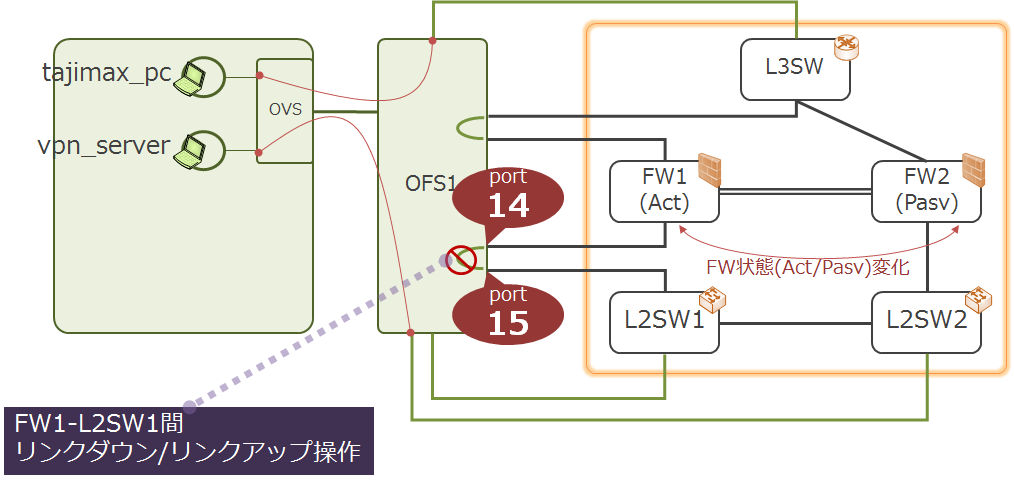
\includegraphics[scale=0.6]{img/poc-env-linkdown.png}
 \caption{PoC環境: NetTesterによるリンクダウン操作}
 \label{fig:poc-env-linkdown}
\end{figure}

  \subsection{継続的通信テストの実装}

テスト対象ネットワークの状態変化を調査する際によく使用されるのは、
Ping(ICMP)を一定間隔で送受信しておき、通信断等の影響がどの程度発生したか
を測定することである。本PoC環境には、L4(TCP)レベルの情報を同期してフェイ
ルオーバー/フェイルバックするFWがあるため、L3(ICMP)レベルでの通信維持確
認に加えて、L4での状態変化通信影響も測定する
(\ref{sec:dynamic-test-target}節)。そのために、TCPセッションを張ったまま
Ping同等の動作をおこなうためのツールを自製
\footnote{\url{https://github.com/net-tester/examples/blob/feature/ood_demo/features/support/echo_server.pl}}
して使用している。

リンク障害発生時のトラフィック影響としては、単純に CIMP/TCP ping ログに
おいてパケットが受信できなかった部分の時間差分を計算する
\footnote{\url{https://github.com/net-tester/examples/blob/feature/ood_demo/features/step_definitions/util.rb},
\code{check\_connection}参照。}ことでおこなっている。

  \subsection{動的なふるまいのテストとして実現できたこと}
  \label{sec:dynamic-test-result}

動的なふるまいのテストとして、ICMP/TCP でトラフィックを継続的に流しなが
らFWのフェイルオーバー・フェイルバックをくりかえすテストを実装することが
できた。PoC環境において、FWフェイルオーバー・フェイルバックの動作で問題
(テスト対象NWの不備)は特に発生しなかった。テスターおよびテストシナリオ実
装上のポイントについては\ref{sec:testscenario-impl-point}節にまとめる。

テストシナリオ実装を通して、ネットワークの通信仕様変更が発生した際の対応
プロセスについても検討している。今回は、\tj からの SSLVPN NAT IP の変更
を題材としている。IP変更要求に対して、以下の手順でテストファーストに対応
を進めるためのデモンストレーション~\cite{nettester-demo-movie}を作成した。
\begin{itemize}
 \item 変更要求にしたがって、対応するテストシナリオを修正する。
 \item テストを実行する。(失敗するテストを書く)
 \item テスト対象ネットワークの設定を変更要求に基づいて変更する。(テスト
       対象の実装)
 \item テストを実行する。(テストが通ることを確認する)
 \item 変更対象のサービス(要求仕様/ふるまい)に影響を与えていないことを確
       認するため、その他のテストシナリオをすべて再実行する。(回帰テスト
       の実行)
\end{itemize}
これにより、要求変化への追従に対するテストファーストな対応、回帰テストに
よる仕様変更対応の影響範囲の調査(予期しない影響が発生していないこと)を実
際に実装し、確認することができた。

 \section{テストシナリオ実装における検討ポイント}
 \label{sec:testscenario-impl-point}

  \subsection{Teardown処理}
  \label{sec:teardown}
CI/CDといったプロセスを実現する上で、複数・任意のテストシナリオをまとめ
て実行することが求められる(回帰テスト含む)。

テストシナリオはいずれも、テスト対象が所定の初期状態にあるところから実行
を開始しなければ狙った「ふるまい」を調査することができない。ソフトウェア
の自動テストでは、テスト対象となるアプリケーション(プロセス)やインスタン
スは初期状態で起動しなおすことが容易なため、常にアプリケーションやインス
タンスを起動しなおして初期状態からのテストをおこなうのが一般的である。

しかし、ネットワーク(特に物理ネットワーク)を対象としている場合はテスト対
象が物理的に存在している。よって、そのままでは、前のテストシナリオ実行直
後のネットワーク状態が次のテストシナリオ実行開始時の初期状態となってしま
う。個々のテストシナリオ実行のたびにネットワーク(機器)の初期化・再構築す
ることは、不可能ではないが以下の理由により難しい。
\begin{itemize}
 \item 機器によっては、コンフィグ消去・再起動に数分から十数分かかるもの
       がある。
 \item 再起動によるteardown処理をおこなう場合、ネットワーク機器の起動順
       序によりネットワーク全体の状態が変化し得る。
 \item コンフィグリセット操作に失敗すると再起動後にリモートアクセスでき
       ず、復旧作業(現地作業)が必要になるリスクがある。
\end{itemize}
特に本PoCでは、静的なふるまいのテストとして数十の通信要件をテストするた
めのシナリオを連続実行したいという要求があるため、単一テストシナリオ実行
の時間的なオーバーヘッドが大きいことが問題となる。

そのため、テストに応じて何らかの形でネットワークの状態を初期状態に戻すた
めの処理(teardown処理)を実装する必要がある。本PoCではL2-L4の状態に着目し
て、以下のteardown操作を実装している。

    \paragraph{テスト対象ネットワークの状態操作}
テスト対象ネットワーク各機器のL2-L4の状態をクリアする(CLIによる各種
\code{clear}コマンドの実行)。
\begin{itemize}
 \item MACアドレステーブル/ARPキャッシュのクリア
 \item FWの NAT Table のクリア
 \item FWの active/standby 状態のクリア
       \begin{itemize}
        \item 今回、動的なふるまいのテストにあたって、FWは障害が発生した
              リンクの復旧にあわせて active/passive を自動復旧するように
              設計したため、特に操作していない
              (\ref{sec:physical_nw_design}節)。
       \end{itemize}
\end{itemize}

    \paragraph{Netns の /etc 配下のSetup/Teardown}
    % 自作echoサーバーで通信開始時に10秒のラグが起きる問題 – NetTester
    % https://3.basecamp.com/3088280/buckets/867009/todos/274457003

NetTesterでは、Network namespace でテスト用ノードを生成する。このときバッ
クエンドでは iproute2(\code{ip}コマンド)を使用している。iproute2 によっ
て生成されたノード(netns)では、\verb|/etc/netns/<netns>/| が etc ディレ
クトリとしてマウントされる~\cite{iproute2-doc}。そのため、テスト用ノード
内部での名前解決などでは、実体としては \verb|/etc/netns/<netns>/hosts|,
\verb|resolv.conf| を参照する。これらの設定ファイル等が正しく設定されて
いないと、名前解決がタイムアウトするなどの問題が発生する。

    \paragraph{物理OFSのflow tableのクリア}
物理OpenFlowスイッチには、テストのたびにフローエントリが登録される。その
ため、テストの実行のたびにフローエントリのクリア処理が必要となる。

本PoCでは、テスト用ノードのMACはテスト実行時にランダムに設定するよう実装
したため、テスト実行をくりかえすと多数の不要なフローエントリが物理スイッ
チ上に残る。テスト用ノードのMACアドレスを固定にすることでフローテーブル
の消費は抑えられるが、異なる用途で同一のMACアドレスを使いまわすなどのケー
スで、予期しない動作不具合が発生する恐れがある\footnote{NetTesterのテー
ブル設計では、テスト用ノードのMACアドレスをキーとして、フロー優先度
(priority)による制御をおこなう(\ref{sec:flow-priority-design}節)。同一
MACアドレスを異なる用途で使いまわす場合、他の用途として設定したフローエ
ントリとマッチしてしまい、狙ったパッチ動作が実現できない恐れがある。}点
に注意すること。

    \paragraph{テスト用ノードのパラメタ設定の考えかた}
    % テスト用ノード(host)のMAC addr を固定にするかどうか方針を決める。 – NetTester
    % https://3.basecamp.com/3088280/buckets/867009/todos/218612153

テスト用ノードのMACアドレス設定による不具合が見付かった際
(\ref{sec:find-nw-device-bug}節)、一時的にテスト用ノードのMACアドレス設
定をテストシナリオ上で固定にすることで回避した。しかし、実際にはteardown
処理を実装し、テスト用ノードのMACアドレスはシナリオ実行時にランダムに設
定されるようにした。これは次のような考えかたによる。
\begin{itemize}
 \item 通常、テスト対象に接続する機器のMACアドレスについて、テスト作業者
       が意識していることはほとんどない。テストシナリオを記述する際にも
       同様に、意識しなくてよいものを意識させなければいけない実装は避け、
       テストシナリオの本質的な部分の実装に注力できるようにすべきである。
       \begin{itemize}
        \item もちろんテストシナリオとして常に指定したMACアドレスを使う
              ことも可能である。テスト対象ネットワーク内の個々の機器につ
              いて、ユニットテストで詳細な動作を調査するような場合にはこ
              うした機能が必要になるが、本PoCでは「ふるまい」つまり要求
              仕様ベースでのテストを主眼においており、そのレベルで本題で
              ないパラメタ設定はテストシナリオ実装者に極力意識させないよ
              うにする。
       \end{itemize}
 \item 物理的なテスト対象では、テスト対象インスタンスの状態を低コストで
       クリアすることが難しく、teardown処理はテスト自動化において重要な
       処理となる。一時的にMACアドレス等の設定で回避してしまうのではなく、
       PoCを実行するうえで実用性があるかどうかを見極める必要がある。
\end{itemize}

  \subsection{NetTesterおよびテストシナリオの並列実行と排他制御}
  \label{sec:testscenario-excl-ctrl}

物理ネットワークをテストする場合、テスト対象(物理ネットワーク)はひとつし
かない。テストの数が多くなる場合、複数のテストを同時に実行することが考え
られるが、現状NetTesterを使ったテスト自動化では、並行実行は原則できない。
以下にその理由を列挙する。

\begin{description}
 \item[状態操作の競合] テストシナリオごとに、想定しているテスト対象ネッ
            トワークの状態がある。それらを変化させるテストシナリオは同時
            に実行できない。
            \begin{itemize}
             \item テストシナリオAを実行している途中で、テストシナリオB
                   がteardown処理を実行して、テスト対象ネットワークの状
                   態クリアをしてしまうと、テストシナリオAで想定していた
                   状態を変化させてしまう\footnote{Teardown処理として
                   \code{clear}コマンドを使用しているが、特定シナリオで
                   使うエントリだけを消去するのではなく、NW機器全体の情
                   報をまとめて消去してしまうため。そのシナリオに依存す
                   るエントリだけをねらって消去できるのであればこの制約
                   は外れるが、テスト対象ネットワーク内の機器それぞれに
                   ついて対応可能かどうかという点が問題となるだろう。あ
                   るいは、teardown処理を他のテストシナリオ実行がおわる
                   まで待機し、まとめて実行できればよいが、現状はそうし
                   た実装をおこなっていない。}。
             \item 動的なふるまいのテストのように、ネットワーク全体の状
                   態に影響をあたえるようなテストシナリオは同時に実行で
                   きない。
            \end{itemize}
 \item[ネットワークリソースの競合] テスト対象ネットワークで一意でなけれ
            ばならないリソースの操作については同時に実行できない。
            \begin{itemize}
             \item テストシナリオA/Bが同じIP/MACを持つテスト用ノードを同
                   時に生成してしまうと、テスト対象ネットワーク内で
                   IP/MACの重複が発生してしまう。
             \item 物理リンクの操作など、ひとつしか存在しないリソースの
                   制御が必要なテストシナリオは同時に実行できない。
            \end{itemize}
\end{description}

本PoCでは\figref{fig:poc-env-physical-detail}のようにふたつのtester set
を使用しているが、これはあくまでもデバッグ用途のためである。Tester set
を複数用意することで、静的なふるまいのテスト(NWが定常状態にある)で、かつ
同じIP/MACのテスト用ノードを使用せず、teardown 処理をテストシナリオ単位
で実行しないようなケースに限って複数のテストが実行可能となる。

上記の制約の一部については、NetTesterで実行されるタスクの排他制御のしく
みを導入することで対応できるものがあるが、現状はそうした対応については本
PoCの範囲外としている。本PoCでは、ひとつのテスト対象ネットワークに対して
tester setがあり、同時にひとつのテストシナリオを実行することが前提となっ
ている。

  \subsection{テストダブルの考えかた}
  % ニセ○○サーバとステップ実装 – NetTester
  % https://3.basecamp.com/3088280/buckets/867009/documents/216490375
一般的に、ソフトウェアテストにおいて、テスト対象が依存しているコンポーネ
ントを置き換える代用品のことをテストダブル~\cite{test-double}という。

本PoCのように、end-to-end のネットワークテストを行なう場合、テストトラ
フィック生成のためにクライアント/サーバを用意する必要がある。テスト対象
ネットワーク内に既存のサーバがあるケースもあれば、本PoCのように実際には
サーバがなく、代替となるサーバをテストシナリオで準備しなければならないケー
スもある。

テストダブルとしてのサーバを導入する場合、導入することによってその他のテ
ストコードの書き換えが発生する(実際のサーバがある場合のテストコードと代
替サーバを使う場合のテストコードが大きく異なる)のは好ましくない。

例として、インターネット検索(google)の可否をテストする場合、テスト対象ネッ
トワークが直接インターネットアクセス可能で直接googleのウェブサイトを見る
ことができる場合、\lstref{lst:real-service-test}のようなステップにできる。
テスト対象ネットワークが直接インターネットアクセスできない場合は、テスト
ダブルを建てて\lstref{lst:testdouble-test}としたとする。

\begin{lstlisting}[caption=実際のサービスを利用する場合,label=lst:real-service-test]
When(/^ブラウザで Google のページを開く$/) do
  cd('.') do
    @browser_pc.exec 'curl -L https://google.com/ > log/google.log'
  end
end

Then(/^Web サイトへのアクセスに成功$/) do
   step %(the file "log/google.log" should contain "<title>Google</title>")
end
\end{lstlisting}

\begin{lstlisting}[caption=テストダブルを利用する場合,label=lst:testdouble-test]
When(/^ブラウザで Google のページを開く$/) do
  cd('.') do
    @browser_pc.exec "nc 192.0.2.100 80 > log/nc_web.log"
  end
end

Then(/^Web サイトへのアクセスに成功$/) do
  step %(the file "log/nc_web.log" should contain "OK")
end
\end{lstlisting}

\lstref{lst:testdouble-test}では、テストダブルを使用することでサーバにつ
いてのコードを変更しているが、それだけでなくクライアント側の処理に関する
コードにも影響をあたえてしまっている。「ふるまい」として「googleに接続し
て検索したい」という目的をふまえると、\lstref{lst:real-service-test}では
直接的に「検索サービスに接続」していることがわかるが、テストダブルを導入
した\lstref{lst:testdouble-test}では、本来テストしたい「ふるまい」を間接
的にしか表現できていない。

しかし実際には、テストダブルで代替したい元のサービスを完全に実現すること
は不可能である(簡単にオリジナルのサーバを準備できるのであればテストダブ
ルを準備する必要がない)。本PoCでは、例えば
\tabref{tab:poc-requires-yo-int} No.1 では git を使用する要件がある。実
際に \verb|git clone|コマンドでリポジトリ操作可能かどうか(L7)というレベ
ルでテストするのか、TCP(L4)レベルの接続性だけをテストするのかなど、テス
トとしてどこまでを保証するのかという線引きをテスト自動化システムのポリシ
として設定しておく必要がある。

  \subsection{コマンドのバックグラウンド実行}
  \label{sec:background-exec-method}
  % コマンドをバックグラウンド実行 – NetTester
  % https://3.basecamp.com/3088280/buckets/867009/documents/216399643
  % step内でのバックグラウンドコマンド実行 – NetTester
  % https://3.basecamp.com/3088280/buckets/867009/todos/202691188

テスト用ノードでのサーバプロセスの実行(テストダブルの生成)、動的なふるま
いのテストにおける複数トラフィックの同時生成などでは、並列でコマンドを実
行する・クライアント操作が終了したらサーバを終了する、などの処理が必要に
なる。単発の同期コマンド実行(\verb|exec|)ではなく、非同期で実行し、join
させるような手段が求められる。

NetTesterを使ったテストステップの実装では、バックグラウンド実行の方法と
して以下のふたつの方法がある\footnote{\code{Netns\#exec}でバックグラウン
ド実行することはできない。これは\code{Netns\#exec}が内部的に利用している
\code{Open3.popen3}の仕様によるものである。}。
\begin{description}
 \item[スレッドを使う] \verb|#exec|自体を別スレッドで動かす。
\begin{lstlisting}
Thread.start { @server.exec "bash -c 'echo OK | nc -l 80'" }
\end{lstlisting}
 \item[直接ipコマンドを使う] \verb|Netns#exec|と同様のことを\verb|ip|コ
            マンドを使って直接バックグラウンド実行する
\begin{lstlisting}
run "sudo ip netns exec #{@server.name} bash -c 'echo OK | nc -l 80 &'"
\end{lstlisting}
\end{description}

本PoCではスレッドを使う方法を採用し、\verb|AsyncExecutor|クラス
\footnote{\url{https://github.com/net-tester/examples/blob/develop/features/support/async_executor.rb}}
を用意してテスト用ノード上でのバックグラウンドコマンド実行をおこなってい
る。

  \subsection{テスト用ノードのパラメタ管理}
  \label{sec:test-parameter-management}
  % factory_girl で仮想ホストを作る – NetTester
  % https://3.basecamp.com/3088280/buckets/867009/documents/210831650

\lstref{lst:nettester_basic_example}で、NetTester の基本的な仕様方法をサ
ンプルコードで示した。NetTester でテスト用ノードを生成する
(\verb|NetTester#new|)場合、テスト用ノードが持つIPアドレス等各種パラメタ
を設定する必要がある。これらのパラメタは複数のテストシナリオにまたがって
使用されたり、テスト結果によっては変更されることがあるため、
\lstref{lst:nettester_basic_example}に示すような直接的なパラメタ記述では
管理が非常に煩雑になってしまう。

そこで、テストデータの管理に Factory Girl~\cite{factory-girl}を使用する。
各テストシナリオで使用するテストデータを
\verb|features/factories.rb|\footnote{\url{https://github.com/net-tester/examples/blob/develop/features/factories.rb}}
で管理する。\verb|factories.rb|では次の情報を記述する。
\begin{description}
 \item[仮想ノード共通属性の定義] ネットワークアドレスやゲートウェイのよ
            うに、各テスト用ノードが共有する属性を記述する。
\begin{lstlisting}
FactoryGirl.define do
  trait :internal_network_host do
    netmask '255.255.255.0'
    gateway '10.10.10.254'
    mac_address Faker::Internet.mac_address('00')
  end

 ...
end
\end{lstlisting}
 \item[仮想ノードの定義] すでに定義した \verb|:internal_network_host| 使っ
            て仮想ノードを生成する。
\begin{lstlisting}
FactoryGirl.define do
  ...

  factory :ntp_client, class: Netns do
    internal_network_host

    name 'ntp_client'
    ip_address '10.10.10.3'
    virtual_port_number 2
    physical_port_number 2
  end
end
\end{lstlisting}
\end{description}

Factory Girl で定義されたテストデータを使用してテスト用ノードを生成する
と次のようになる。このように、テスト用ノードの共通パラメタを分離し、パラ
メタの設定や管理を効率的に実装することができる。
\begin{lstlisting}
Given(/^NTP クライアントとなる開発者 PC$/) do
  @ntp_client = Netns.new(attributes_for(:ntp_client))
end
\end{lstlisting}

  \subsection{テストシナリオのサイズ}

% シナリオサイズの目安、シナリオ分割の目安 (step3 test つくっているときに
% 分割するって話になった理由は?)
% Answer to “今日なにした?” – NetTester
% https://3.basecamp.com/3088280/buckets/867009/question_answers/267488304
% 集中作業日1 – NetTester
% https://3.basecamp.com/3088280/buckets/867009/schedule_entries/260224157

動的なふるまいのテスト(リンク障害試験)について、手作業で実施する場合には、
1回のイベント(リンクダウンまたはリンクアップの発生)に対して複数の操作を
おこなう。例えば、あらかじめ複数のテストトラフィックを生成しておき(今回
のPoCシナリオでは複数パスの ICMP/TCP pingの実行)、1回のイベントに対して
それらのトラフィックがどう変化したのかを確認する。

これをそのままテストシナリオとして記述すると、ひとつのシナリオのステップ
数が増大し、テストシナリオ全体の見通しが悪くなってしまう。そこで本PoCで
は、テストが繰り返し実行可能であることを利用して、イベント・トラフィック
ごとにテストのシナリオを分割し、ひとつひとつのテストシナリオが単純かつ理
解しやすいものになるようにした。

手作業でテストシナリオを実行する場合には、くりかえし実行(作業)する時間的
コストが大きいためイベントの発生回数自体をおさえる。しかし、テストシナリ
オを自動化した場合は、繰り返し実行することのコストは低い。そのため手作業
で実行する際の一般的なやりかたに準拠させる必要はなく、個々のテストシナリ
オのメンテナンス性を重視して考えることができる。

  \subsection{Sleep tuning}
  \label{sec:sleep-tuning}
% step3 テストにおけるsleep調整など、課題、対応について。

テストシナリオ(テストステップ)の実装にあたっては、処理のタイミングを同期
させるために sleep によるタイミング調整が必要になる。
\begin{itemize}
 \item 処理の待機
       \begin{itemize}
        \item 物理OFSとOFCとの接続・再接続の待機
        \item テスト対象機器に対するコマンドの発行、処理実行の待機
        \item コマンド実行後のログファイル生成等の待機
        \item スレッドによるコマンドの同時実行
              (\ref{sec:background-exec-method}節)を使用する場合は、スレッ
              ドのスケジューリングのためにコマンド実行までにタイムラグが
              あるため sleep を設定する。
       \end{itemize}
 \item テストシナリオ上必要な操作タイミング設定
       \begin{itemize}
        \item 動的なふるまいのテストの場合は、イベント発生前・発生後の定
              常状態遷移待機(テスト対象ネットワークのトポロジの収束など)
              のように、テスト対象の状態変化にかかる時間にあわせたテスト
              オペレーション実行タイミング調整が必要になる。
       \end{itemize}
\end{itemize}

テストシナリオ上必要なタイミング設定についてはテストステップとして明示的
にテストシナリオ中に待機時間を明示する。
\begin{lstlisting}
When(/^(\d+) 秒待つ$/) do |seconds|
  sleep seconds.to_i
end
\end{lstlisting}

処理の待機について、テストシナリオの実行と本質的に無関係のものであればテ
ストシナリオ上は明示させる必要がない。テストステップ中での sleep 実装は
意図や必要性がわかりにくくなりがちであるため乱用には注意が必要である。ま
た、デバッグのために一時的にsleepを設定することがある(一時的にテストシナ
リオ実行を遅延させて別途テスト対象ネットワーク上での調査や作業をおこなう)よ
うなケースでは不要なsleepチューニングが残らないようにする必要がある。

  \subsection{標準出力(stdout)の操作}
  % 今日なにした? – NetTester
  % https://3.basecamp.com/3088280/buckets/867009/questions/181826801/answers/2016-10-21#__recording_267488304
テストステップ実装では、テスト用ノードのコマンド実行結果(stdout)を取得し
たいケースがある。このとき、\verb|$stdout|の操作をおこなってしまうと、
teardown処理等で実行するexpect系ツールへ影響を与えてしまうことがある。

今回、テスト対象ネットワークの操作にはexpectacle(\ref{sec:expectacle}節)
を使用しているが、内部的には \code{spawn} されたコマンド
d(\code{telnet},\code{ssh})の標準出力を\code{pty}/\code{expect}で操作して
いる。テストシナリオ(テストステップ)側で \verb|$stdout| などを操作してし
まうと、こうしたプロセスに影響が及んでしまう点に注意すること。

 % \section{テストシナリオのリファクタリング}
 % TODO
 % というかまだおわってないのでこれはいったん省くか

 \section{テストシナリオのデバッグ}

テストシナリオの実装・実行をした際、テストが失敗したときには原因として以
下の要因が考えられる(\ref{sec:statictest-founded-issues}節)。また、これ
らの原因が複合して発生することがある。
\begin{description}
 \item[テストシナリオ実装とテスト対象ネットワーク実装の認識違い] テスト
            実装者とテスト対象ネットワーク構築者との認識違い。
 \item[テスト対象ネットワークの設計や設定の不備] テストの目的通り、テス
            ト対象が仕様を実現できていないこと、予期しない動作を発見でき
            ている状態。
 \item[テストシナリオの実装上の不備] テストシナリオ・テストステップ実装
            上の不備。テストに仕様するツールやコマンドの実行時エラーやシ
            ナリオ全体としてみたときのテストオペレーション実行タイミング
            のずれ・ログ取得不備など。
 \item[テスター(NetTester)の動作不具合] NetTester実装においてはテスター
            自体の動作の問題やバグなどが発生する。
\end{description}

% 原因切り分けのメモを書く – NetTester
% https://3.basecamp.com/3088280/buckets/867009/todos/214926110
% 原因切り分けメモ (muraki) – NetTester
% https://3.basecamp.com/3088280/buckets/867009/documents/217782147

テストが失敗した場合は、まずは問題がテスター側にあるのかテスト対象ネット
ワーク側にあるのかを切り分ける必要がある。以下に問題切り分け・デバッグ時
の確認ポイントを示す。
\begin{itemize}
 \item テスト対象ネットワーク側での操作
       \begin{itemize}
        \item ARP/MACアドレステーブルの確認: テスト用ノードが生成したト
              ラフィックがテスト対象ネットワークに届いているかどうかを確
              認する。テスター側のVLAN設定とテスト対象ネットワーク機器側
              のポートVLAN設定とのミスマッチに注意すること。
        \item テスト用ノード接続ポートのパケットカウンタ(エラーカウンタ
              の確認)
        \item パケットキャプチャ: テスト対象ネットワーク機器でテスト用ノー
              ドが生成したトラフィックが送受信できていない場合はパケット
              キャプチャしてヘッダ等の情報を確認する。(NetTesterの場合、
              L2(MAC, VLAN Tag)の操作をおこなうので注意。)
       \end{itemize}
 \item テスター側OVSでの操作
       \begin{itemize}
        \item OVSのポート通信量の確認: テスト対象ネットワーク機器側とあ
              わせて確認することで、L1/L2レベルでの接続状態確認を実施す
              る。
\begin{lstlisting}
ovs-ofctl dump-ports <bridge> <port-number>
\end{lstlisting}
        \item フローテーブル、フローエントリに対するパケットカウンタの確
              認: フローテーブル設計・実装のデバッグをおこなう
              \footnote{2016年12月時点では、NetTesterはOFSのteardown処理
              を実装していない。過去のテストの際にフローテーブルに残った
              エントリによる影響なども考慮に入れる必要がある
              (\ref{sec:teardown}節)。}。
\begin{lstlisting}
ovs-ofctl dump-ports <bridge>
\end{lstlisting}
        \item OFS-OFC間通信(セキュアチャネル)状態
       \end{itemize}
 \item テスター(NetTester)サーバでの操作
       \begin{itemize}
        \item PSW-SSW間リンクでのパケットキャプチャ: NetTesterサーバの
              OFSスイッチ間接続用物理ポート
              (\figref{fig:nettester-deploy-vm}のens5相当のインタフェー
              ス)ですべてのテスト用ノードがやりとりするトラフィックをキャ
              プチャできる。
        \item テスト用ノードの ARP テーブルの確認
        \item NetTester OFC(trema)でのデバッグ:
              \ref{sec:debugging-trema}節参照。
        \item OS上での不要な network namespace や veth インタフェース等
              の確認
       \end{itemize}
 \item テストシナリオでの操作
       \begin{itemize}
        \item Pry~\cite{pry}によるデバッグ: テストシナリオ(ステップ)中に
              pry を挿入することで、シナリオ中の特定の箇所でインタラクティ
              ブシェルに以降し、テストシナリオ上の変数やテスト対象ネット
              ワークの状態などを確認する。
        \item 各テストオペレーションでの操作ログの取得
        \item Sleep tuning, テストシナリオの連続(繰り返し実行)や実行間隔
              の調整: キャッシュ依存の動作やタイマベースの状態変化イベン
              トなどでは、テストの実行タイミングあるいは実行順序によって
              テスト実行結果が変化することがある。
       \end{itemize}
\end{itemize}

こうした作業では、テスター側の動作状況・ログだけでなく、テスト対象ネット
ワーク内の各機器に対するオペレーションや状態変化ログもあわせて一元管理で
きることが望ましい。そのために、一般的なネットワークのテスト実行や検証作
業と同様、テスト対象ネットワーク機器のログ(Syslog)の収集、時刻同期(NTP)
などを実施しておくことが必要である。この他、テスト環境としては以下のよう
な点が検討事項となる。
\begin{itemize}
 \item テスト自動化として物理構成操作を極力避けたいという狙いがあるため、
       テスト環境構成の際にはあらかじめ、パケットキャプチャのためのリソー
       スや予備配線などを想定した設計をしておくことが望ましい。
 \item 問題切り分け用の対照設定・対照機器の準備: 今回テストシナリオ実装
       にあたっては、FWのパケットフィルタを設定していない(permit any)FW
       を1台用意し、テスト用ノード(server/client)が直接通信してテストが
       実行可能かどうかを切り分けられるようにした。テストシナリオを一度
       に作成してテスト実行可否を見極めるのが難しい場合は、段階的なテス
       トシナリオ自体の動作確認や切り分けが可能な工夫が求められる。
\end{itemize}

\section{PoC結果に関する定性的な評価}
% 評価・考察
% - 体制や役割分担/タスクとスキルセットについて
%   https://3.basecamp.com/3088280/buckets/867009/todos/260220903
% - テスト実装のコスト
% - 繰り返し実行できることのメリット
%   - OSの更新などおおきな変更にたいするリスクヘッジ

本PoCでは、BDDの考えかたのもとに、静的・動的なふるまいのテストを実装した。
実際に、これまで手作業でおこなってきたのと同等の end-to-end 通信試験やリ
ンク障害試験を自動化することができた。また、teardown処理の難しさなど、ソ
フトウェア開発における自動テストでは存在しない(物理ネットワークのテスト
固有の)問題などもあきらかにすることができた。本節ではテスト自動化システ
ムの運用に付随する検討事項や当初目的に対する今後の課題について解説する。

  \subsection{ネットワークの構築・運用プロセス}

本プロジェクトの目的としてはネットワークの構築・運用プロセスのCI/CD化
(\ref{sec:network-test-and-process}節)がある。今回、
\ref{sec:dynamic-test-result}節に示したように、テストファーストな運用と
いう観点での操作を実際に試している。この中で、テストシナリオによる回帰テ
ストの実行と影響範囲のチェックはできている。CIのための最も基本的なオペレー
ションについては実現性が見えているが、より高度なCIプロセスへ発展させるた
めには、今後下記のような点の検討が必要と考えられる。

    \paragraph{開発プロセスと自動テスト実行}
ソフトウェア開発におけるCIでよく実施されるベストプラクティスに、コードコ
ミット等のイベントをトリガとして自動的にビルド・回帰テストを実行すること
がある。テストシナリオの開発(シナリオの修正や追加)、テスト対象ネットワー
クの実装(設定変更等)に応じて、同様にテスト対象ネットワークを自動構成、テ
スト自動実行をおこなうような仕組みやプロセスが必要になると予想される。

少なくとも、テスト対象ネットワークの構成や設定情報、テストシナリオの開発
プロセスとして、作成・作成者によるテスト、レビュー・レビュアーによるテス
ト、試験環境側でのマージ、本番デプロイなどのフェーズわけやテスト実行のた
めの仕組み(\ref{sec:testscenario-excl-ctrl}節)などの整備が必要となる。

    \paragraph{テスト対象ネットワークの自動構築・操作}
上記のようなCI開発プロセスを想定すると、テスト対象ネットワークの構成(ト
ポロジや設定等)自体をバージョンコントロールし、任意の時点・構成・設定・
状態に巻き戻したうえでテストを実行するような仕組みが求められる。

テスト対象が物理実体、すなわち物理ネットワークを想定すると、こうした任意
の状態操作は難しい。また、テスト対象がひとつに制限されることによる同時テ
スト実行回避(排他制御)など、一般的なソフトウェア開発では発生しない要求な
どを考慮する必要がある。

状態のコントロールとして、現状はteardown処理による初期化をおこなっている
が、特定の障害がおきた状態に戻すなど、指定した状態への復帰が簡単にできる
ようになると、テストシナリオのデバッグ、あるいはテスト対象ネットワークの
デバッグ(再現試験)などへの応用がよりしやすくなると考えられる。

  \subsection{役割分担・スキルセット}

テスト対象ネットワークの設計・構築、テストシナリオの実装・テストの実行に
あたって、\tabref{tab:skillset}のような役割・スキルセットが求められる。
テスター(NetTester)自体の開発やデバッグでは、
Ruby/Trema/OpenFlow/OpenFlow Switch等の知識が求められるが、テストシナリ
オの策定や実装については一般的なネットワークの知識とある程度のプログラミ
ングの知識\footnote{Cucumberとrubyによるテストステップの実装: 数行-数十
行のrubyスクリプトが作成できるレベル。本PoCのシナリオでは、外部コマンド
実行や結果の取得・パースなどがrubyで実装できればよい。}があれば対応が可
能である。

実際に各テストシナリオ・テストステップ実装を進めるにあたっては、個々のテ
ストシナリオ担当者のプログラミングスキルというよりは、テストシナリオ全体
の方針設計、レビューなどによるテストシナリオ実装の品質のコントロールがで
きることが重要だった。特に、ネットワークエンジニア観点でのテストシナリオ
実装をおこなうと、ユニットテストに近いテストシナリオや仕様ベースではなく
NW機器の知識をベースにしたテストシナリオを実装してしまう(過剰・冗長なテ
ストを実装してしまう)傾向が見られた。また、テストシナリオやテストステッ
プ間の機能重複の排除、ファイル構成の見直しなど、テストシステム全体のリファ
クタリングの検討などをするうえでも、ソフトウェアによるテスト自動化のノウ
ハウが必要となる。「ネットワークのBDDとして必要十分なテストは何か」をコ
ントロールするために、テスト自動化についての知識や経験を持ち、テストシナ
リオのありかた・方向性を設定できるソフトウェアエンジニアがいることが望ま
しい。

\begin{table}[h]
 \centering
 \caption{テストシナリオ実装で求められる役割とスキルセット}
 \label{tab:skillset}
 \begin{tabular}[t]{p{15zw}|p{30zw}}
  \hline
  役割 & スキル \\
  \hline
  \hline
  テストシナリオ内容の決定 & テスト対象ネットワーク仕様の理解; シナリオ作成担当に対するシナリオ仕様を決定する(feature fileレベルのシナリオの策定) \\ \hline
  テスト対象NWの整備 & テスト対象ネットワーク仕様の理解; テスト対象ネットワークの設計・構築 \\ \hline
  テスターおよびテストシナリオ開発環境の整備 & テスト対象ネットワーク構成(物理構成)の理解; テスター(NetTester)のデプロイとメンテナンス; テストシステム構成情報をシナリオ作成担当へ渡す \\ \hline
  シナリオ作成 & NetTester APIの理解; Ruby/Cucumberの理解; テストシナリオ(feature)の理解; テストステップの実装 \\ \hline
  シナリオ実行 & テストシナリオの実行; テスト対象ネットワーク仕様の理解; テスト結果の判断 \\ \hline
  物理環境の操作・調査 & テスト対象ネットワーク側原因調査(デバッグ); ネットワーク機器の操作・設定変更 \\ \hline
  テストシナリオ実装の調査 & テストシナリオ側原因調査(デバッグ) \\ \hline
  テスター実装の調査 & テスター側原因調査(デバッグ) \\ \hline
 \end{tabular}
\end{table}

  \subsection{テストシナリオの実装コスト}

テスト自動化に限らず「自動化」システムはイニシャルの実装コストがどうして
も発生してしまう。また、テスト自体もシステムの変化にあわせて更新・修正し
ていく必要があり、そうしたメンテナンスコストについても検討が必要になる。

参考までに一部のテストシナリオ実装事例についての開発コスト指標を以下に示
す。ただし、本PoCではゼロからのテストシナリオ検討およびテスター
(NetTester)自体の開発を並行して実施しているため、テストシナリオ実装の一
般的な初期コストとして直接利用できる値ではない。
\begin{description}
 \item[静的なふるまいのテストの実装コスト] テストシナリオ方針がきまって、
            テストステップの共通項目がそろってきた後半でのシナリオ開発で
            は、ひとつの通信要件に対するテストシナリオの実装に0.5-1.0人
            日程度が必要だった。テストツールでの確認を複雑にする(L7レベ
            ルの動作を見る)ようなケースでは、テストで使用するツール(コマ
            ンド)に関する予備知識の有無などで実装コストは変動する。
 \item[動的なふるまいのテストの実装コスト] 最初の1シナリオの構築にあたっ
            ては、NW機器設定の担当者・テストシナリオ実装の担当者をそろえ
            て実際の動作を見ながら実装を進める必要がある。初回実装では、
            動的なテストを手動で実行するのと同等のオペレーションと、それ
            を自動化するための知見や調整\footnote{Sleep Tuning
            (\ref{sec:sleep-tuning}節)やSyslog等によるテスト結果判定の実
            装など。}が必要であり、2-4人日程度を要した。一度基本となるシ
            ナリオが実装できて動作確認がとれると、あとは基本シナリオの応
            用となって1シナリオ0.5-1.0人日程度で実装できた。
\end{description}

%%% Local Variables:
%%% mode: yatex
%%% TeX-master: "main.tex"
%%% End:
